Using the results gathered from the experiments, we set out to create one that was better than what we got there. We saw that there were quite a few things that improved the performance of the model. The things we decided seemed most crucial was adding a second layer with dropout, and increasing the number of hidden features in the model. Our model ended up with the following hyperparameters:
\begin{itemize}
    \item Character embedding size: 30
    \item Starting learning rate: $8e-4$
    \item Learning rate schedule: Multiply by $0.2$ every 5 epochs
    \item Layers: 2
    \item Hidden layer size: $600$
    \item Training time: 15 epochs/8 hours
\end{itemize}
Unfortunately, this model did not end up outperforming the best model from the experiments, and due to time constraints, we could not train another. The resulting plots can be seen in Figure ~\ref{fig:finished_tsne} and ~\ref{fig:finished_spearman}

\begin{figure}[!ht]
  \centering
  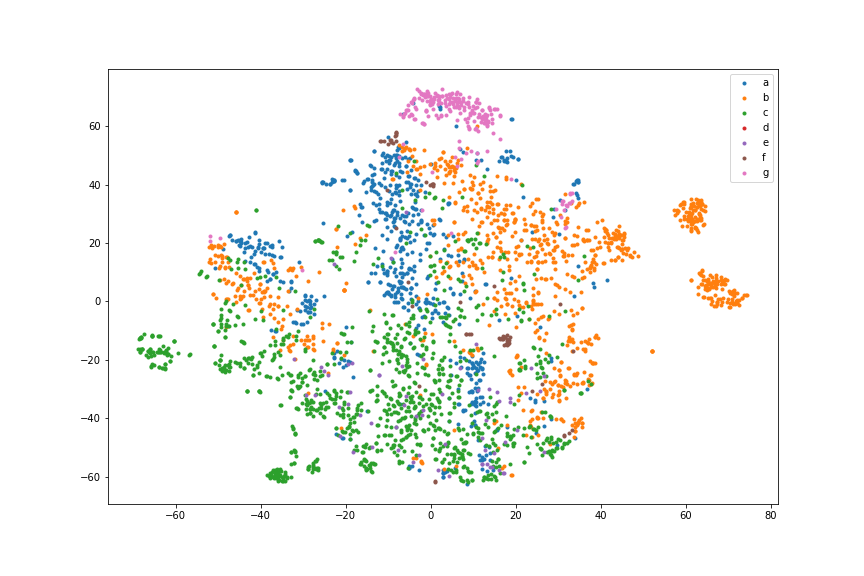
\includegraphics[width=0.49\linewidth]{latex/imgs/finished_tsne_final.png}
  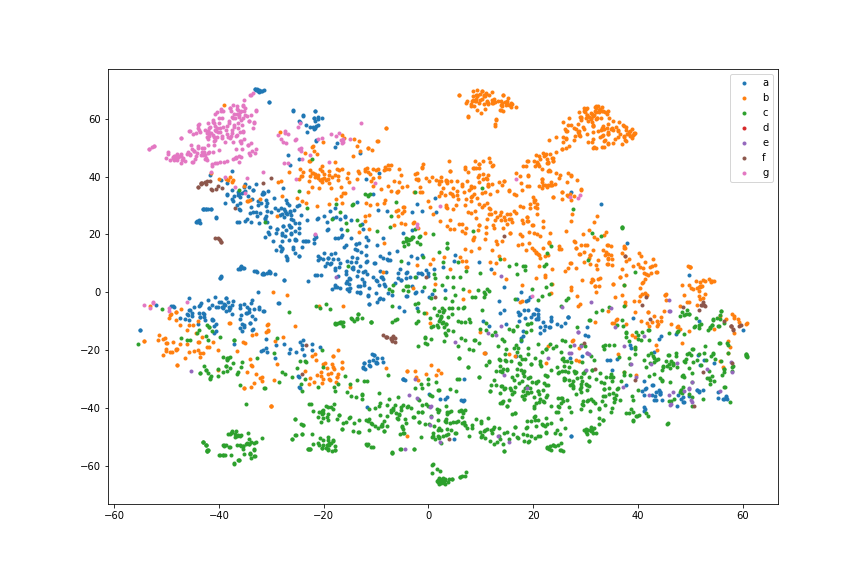
\includegraphics[width=0.49\linewidth]{latex/imgs/finished_tsne_minloss.png}
  \caption{The TSNE plots generated from the last model. Left is final, right is minloss.}
  \label{fig:finished_tsne}
\end{figure}

\begin{figure}[!ht]
  \centering
  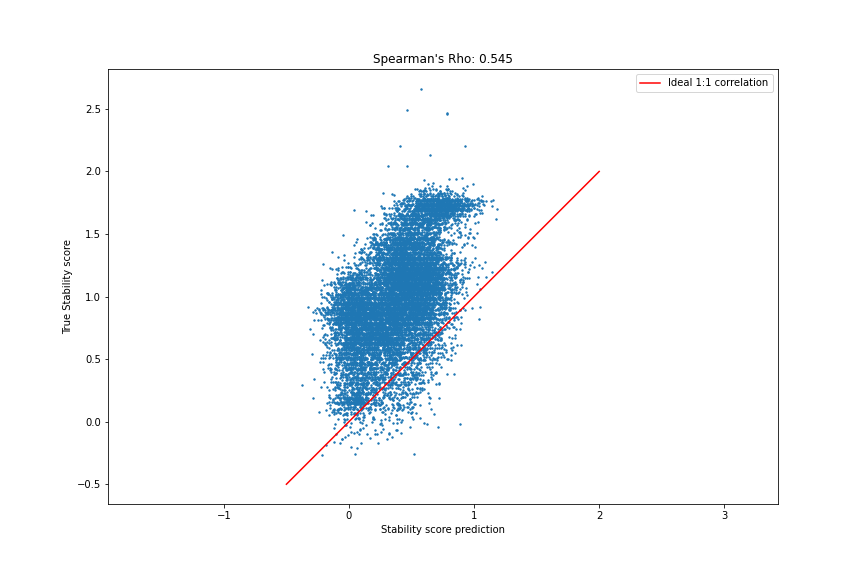
\includegraphics[width=0.49\linewidth]{latex/imgs/finished_spearman_final.png}
  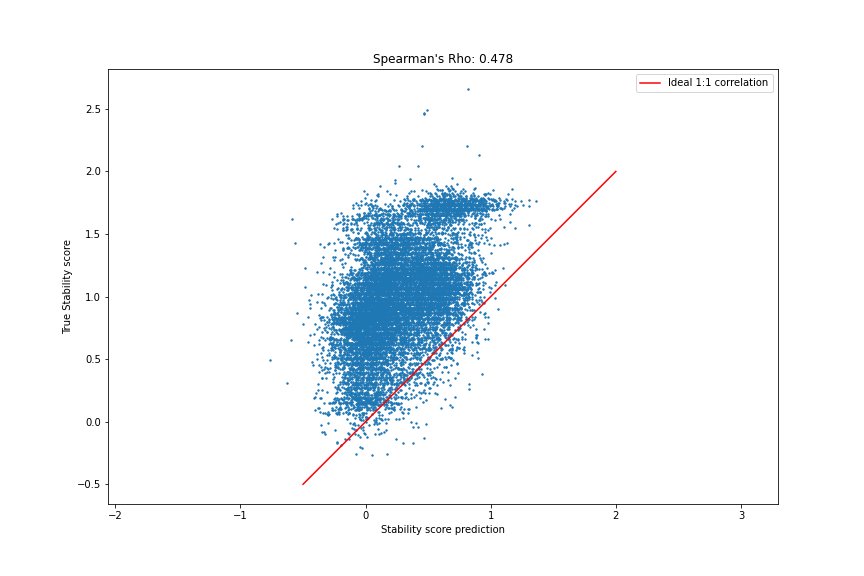
\includegraphics[width=0.49\linewidth]{latex/imgs/finished_spearman_minloss.png}
  \caption{Spearman plots generated from the last model. Left is final, right is minloss.}
  \label{fig:finished_spearman}
\end{figure}